%% Based on a TeXnicCenter-Template by Tino Weinkauf.
%%%%%%%%%%%%%%%%%%%%%%%%%%%%%%%%%%%%%%%%%%%%%%%%%%%%%%%%%%%%%

%%%%%%%%%%%%%%%%%%%%%%%%%%%%%%%%%%%%%%%%%%%%%%%%%%%%%%%%%%%%%
%% HEADER
%%%%%%%%%%%%%%%%%%%%%%%%%%%%%%%%%%%%%%%%%%%%%%%%%%%%%%%%%%%%%
\documentclass[a4wide,twoside,11pt]{report}
% Alternative Options:
%	Paper Size: a4paper / a5paper / b5paper / letterpaper / legalpaper / executivepaper
% Duplex: oneside / twoside
% Base Font Size: 10pt / 11pt / 12pt


%% Language %%%%%%%%%%%%%%%%%%%%%%%%%%%%%%%%%%%%%%%%%%%%%%%%%
\usepackage[french]{babel} %francais, polish, spanish, ...
\usepackage[T1]{fontenc}
\usepackage[ansinew]{inputenc}

\usepackage{color}
\usepackage{listings}
\lstset{language=C,captionpos=b,                   % sets the caption-position to bottom
breaklines=true,float=htbp}
\definecolor{darkgray}{rgb}{0.95,0.95,0.95}
\lstset{backgroundcolor=\color{darkgray}}

\def\ctilde{\scalebox{2}{\kern .3em\lower 1ex \hbox{\~{}} }}
\usepackage{fullpage}

\usepackage[rightcaption]{sidecap}
%\usepackage{lmodern} %Type1-font for non-english texts and characters


%% Packages for Graphics & Figures %%%%%%%%%%%%%%%%%%%%%%%%%%
\usepackage{graphicx} %%For loading graphic files
%\usepackage{subfig} %%Subfigures inside a figure
%\usepackage{tikz} %%Generate vector graphics from within LaTeX

%% Please note:
%% Images can be included using \includegraphics{filename}
%% resp. using the dialog in the Insert menu.
%% 
%% The mode "LaTeX => PDF" allows the following formats:
%%   .jpg  .png  .pdf  .mps
%% 
%% The modes "LaTeX => DVI", "LaTeX => PS" und "LaTeX => PS => PDF"
%% allow the following formats:
%%   .eps  .ps  .bmp  .pict  .pntg


%% Math Packages %%%%%%%%%%%%%%%%%%%%%%%%%%%%%%%%%%%%%%%%%%%%
\usepackage{amsmath}
\usepackage{amsthm}
\usepackage{amsfonts}
\usepackage[colorlinks=true]{hyperref}
\usepackage[normalem]{ulem}


%% Line Spacing %%%%%%%%%%%%%%%%%%%%%%%%%%%%%%%%%%%%%%%%%%%%%
%\usepackage{setspace}
%\singlespacing        %% 1-spacing (default)
%\onehalfspacing       %% 1,5-spacing
%\doublespacing        %% 2-spacing


%% Other Packages %%%%%%%%%%%%%%%%%%%%%%%%%%%%%%%%%%%%%%%%%%%
%\usepackage{a4wide} %%Smaller margins = more text per page.
%\usepackage{fancyhdr} %%Fancy headings
%\usepackage{longtable} %%For tables, that exceed one page


\newenvironment{definition}{{\bf Definition: } \itshape }{\normalfont\vspace{0.8cm}}
\newenvironment{theoreme}{{\bf Theorem: } \itshape\large }{\normalfont\normalsize\vspace{0.8cm}}

\renewcommand{\arraystretch}{1.8}

%\renewcommand{\chaptername}{Lecture}

%\renewcommand{\chaptermark}[1]{\markboth{\chaptername~\#\thechapter~:
%\ #1}{}}
\newfont{\scaledfont}{cmr12 scaled 4000}
\renewcommand{\thechapter}{\arabic{chapter}}
\makeatletter
\def\@makechapterhead#1{
  {\parindent \z@ \raggedright \normalfont
    \interlinepenalty\@M
    \parbox{0.35\textwidth}{\scaledfont{Chap \thechapter:}}\hfill   {\Huge \bfseries #1}
\par\normalsize%
    \rule{\textwidth}{1pt}%  <--- the rule
    \nobreak
    \vskip 40\p@
  }%
}
\makeatother


%%%%%%%%%%%%%%%%%%%%%%%%%%%%%%%%%%%%%%%%%%%%%%%%%%%%%%%%%%%%%
%% DOCUMENT
%%%%%%%%%%%%%%%%%%%%%%%%%%%%%%%%%%%%%%%%%%%%%%%%%%%%%%%%%%%%%
\begin{document}

\pagestyle{empty} %No headings for the first pages.


%% Title Page %%%%%%%%%%%%%%%%%%%%%%%%%%%%%%%%%%%%%%%%%%%%%%%
%% ==> Write your text here or include other files.

%% The simple version:
\title{L'art de programmer son copeau de silicium}
\author{4-AE/I release 2010a}
%\date{} %%If commented, the current date is used.
\maketitle

%% The nice version:
%\input{titlepage} %%You need a file 'titlepage.tex' for this.
%% ==> TeXnicCenter supplies a possible titlepage file
%% ==> with its templates (File | New from Template...).


%% Inhaltsverzeichnis %%%%%%%%%%%%%%%%%%%%%%%%%%%%%%%%%%%%%%%
\tableofcontents %Table of contents
\cleardoublepage %The first chapter should start on an odd page.

\pagestyle{plain} %Now display headings: headings / fancy / ...

\chapter{On en tient une couche}

\section{Charabia et wikipedia}

Un \href{http://fr.wikipedia.org/wiki/Pilote_informatique}{pilote informatique} (ou plus connu sous l'anglicisme \og driver \fg) est un programme informatique qui permet � un autre programme d'interagir avec un p�riph�rique. En g�n�ral, chaque p�riph�rique a son propre pilote.

Pour assurer \href{http://fr.wikipedia.org/wiki/Qualit�_logicielle}{la qualit� d'une application}, il est n�cessaire de bien concevoir les pilotes et leur relation avec l'application. Petit rappel : en informatique, la qualit� d�signe un ensemble d'indicateurs pour offrir une appr�ciation globale d'un logiciel. Elle se base sur : la compl�tude des fonctionnalit�s, la pr�cision des r�sultats, la fiabilit�, la tol�rance aux pannes, la facilit� et la flexibilit� de son utilisation, la simplicit�, l'extensibilit�, etc.

Parmi ces crit�res, le n�ologisme \href{http://fr.wikipedia.org/wiki/Portabilit�_(informatique)}{portabilit�} d�signe, pour un programme informatique, sa capacit� � fonctionner dans diff�rents environnements d'ex�cution, en particulier diff�rents environnements mat�riels. A cela s'ajoute l'\href{http://fr.wikipedia.org/wiki/Adaptabilit�}{adaptabilit�} qui est souvent utilis� pour d�signer la qualit� d'un logiciel qui peut �tre modifi� ais�ment en harmonie avec les changements auxquels son utilisation peut �tre soumise.

La portabilit� et l'adaptabilit� d'une application n�cessite d'avoir une \href{http://fr.wikipedia.org/wiki/Architecture_logicielle}{architecture logicielle} solide. Celle-ci d�finit l'organisation interne d'un logiciel, son d�coupage en couches et en modules, ainsi que les responsabilit�s de chaque module et la nature et la structure des relations entre modules.

Les relations entres les modules sont fournies via une \href{http://fr.wikipedia.org/wiki/Interface_de_programmation}{interface de programmation} (\emph{Application Programming Interface ou API}). Elle permet l'interaction des programmes les uns avec les autres. Du point de vue technique une API est un ensemble de fonctions, proc�dures ou classes mises � disposition par une biblioth�que logicielle, un syst�me d'exploitation ou un service. La connaissance des API est indispensable � l'\href{http://fr.wikipedia.org/wiki/Interop�rabilit�}{interop�rabilit�} entre les composants logiciels.

Dans le cas typique d'une biblioth�que, il s'agit g�n�ralement de fonctions consid�r�es comme utiles pour d'autres composants.
Une interface en tant que telle est quelque chose d'abstrait ; les composants r�alisant celle-ci �tant des mises en {\oe}uvre (ou impl�mentation). Id�alement il peut y avoir plusieurs mises en {\oe}uvre pour une m�me interface. Par exemple, sous UNIX, la libc d�finit des fonctions de base utilis�es par pratiquement tous les programmes et est fournie par des mises en {\oe}uvre propri�taires ou libres, sous diff�rents syst�mes d'exploitation.

\section{Architecture logicielle recommand�e}

Pour en revenir � nos moutons �lectroniques, nous pr�conisons pour les TP de p�riph�riques une architecture logicielle en trois couches (voir figure~\ref{fig:archi}). 

\begin{figure}[!h]
\begin{center}
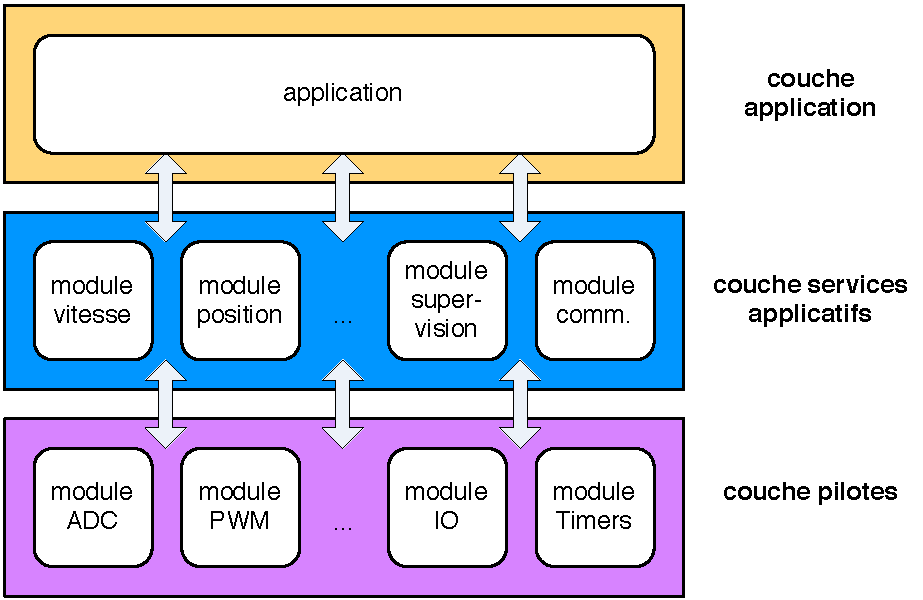
\includegraphics[scale=0.7]{figures/architecture.pdf}
\caption{Architecture logicielle}
\label{fig:archi}
\end{center}
\end{figure}

Les diff�rentes couches sont :
\begin{itemize}
\item {\bf La couche application} : Cette couche ne comporte que du code d�di� � une application. Elle comporte l'ensemble des fonctions de traitement et d'orchestration de l'application. 
\item {\bf La couche de services applicatifs} : Cette couche un ensemble de fonctions qui masquent les p�riph�riques mat�riels au niveau de l'application pour en offrir une repr�sentation abstraite. Par exemple, le service d'acquisition d'une vitesse masque l'appel au p�riph�rique ADC pour offrir une vision purement abstraite de la variable de vitesse. 
\item {\bf La couche de pilotes} : Cette couche ne comporte que du code li� � la configuration et l'utilisation des p�riph�riques sans pr�suppos� une utilisation particuli�re par une application.
\end{itemize}

Une telle architecture offre de nombreux avantages :
\begin{itemize}
\item  Seules les couches \og services applicatifs \fg et \og pilotes \fg doivent changer si le mat�riel �volue, la couche application n'ayant a priori besoin que de quelques modifications pour prendre en consid�ration les nouvelles capacit�s du support d'ex�cution (surtout en ce qui concerne le temps).
\item Les modules qui composent la couche pilotes peuvent �tre utilis�es pour diff�rentes applications et ainsi offrir des composants pris sur �tag�res.
\item La couche services applicatifs fournit des services g�n�riques pour un m�me ensemble de familles d'applications sans avoir besoin d'�tre r��crit � chaque d�veloppement ou �volution d'une application sur le m�me support.
\item Le test des modules est fait de mani�re unitaire, ce qui facilite le d�bogage sans avoir besoin de chercher la petite b�te.
\end{itemize}

Les �l�ments qui composent une couche ne peuvent communiquer qu'avec un �l�ment d'une couche inf�rieure et cela se fait uniquement � travers les API des diff�rentes modules.

\section{Guide des bonnes mani�res}


Chaque module est associ� � deux fichiers, l'un comportant le code (.c) et l'autre d�finissant son API (.h). Seul les fonctions d�clar�es dans le ficher d'en-t�te sont accessibles aux autres �l�ments logiciels.

Comme le fichier d'en-t�te est le seul �l�ment utilisable (lisible / modifiable) par un utilisateur externe au module, il est capital de bien le commenter. Le commentaire est consid�r� comme un mode d'emploi du module. Ceci est d'autant plus vrai, que les constructeurs de micro-contr�leurs proposent des modules (ou biblioth�ques) au format .lib ou .o.  Ces derniers sont compil�s donc de fait, non modifiables.

Afin d'assurer la portabilit� des modules de la couche pilotes, il est interdit qu'une des fonctions d'un module utilisent une variable globale au projet. Si on veut utiliser une variable globale au projet, dans la couches service ou application, cela peut se faire par le biais d'un fichier d'ent�te partag�, par exemple, global.h. Ceci �tant, c'est fortement d�conseill�.

Quelques r�gles sont sp�cifiques aux couches :
\begin{itemize}
\item {\bf Couche application}
	\begin{itemize}
		\item Le \texttt{main()} est contenu dans la couche application et ne peut faire appel qu'� des fonctions de la couche services. 
		\item Aucune r�f�rence � des p�riph�riques n'est fait au niveau de la couche application.
	\end{itemize}
\item {\bf Couche services applicatifs}
	\begin{itemize}
		\item Le code des modules de la couches services contient des fonctions directements li�es � l'application : les noms de fonctions et de variables font explicitement r�f�rence � l'application. 
		\item Les fonctions au niveau services appellent uniquement des fonctions de niveau pilotes. Elles ne s'appellent pas entre elles. Dit autrement, elles ne peuvent inclure que des fichiers de niveau pilote.
		\item Les fichiers sont organis�s par domaine li� � l'application 
	\end{itemize}
\item {\bf Couche pilotes}
	\begin{itemize}
		\item La couche pilotes ne contient que les fonctions qui concernent directement les p�riph�riques.
		\item Les noms des fonctions doivent �voquer les p�riph�riques.
		\item Les fonctions ne font pas r�f�rence � l'application et doivent �tre d�finie de mani�re ind�pendante � toute application.
	\end{itemize}
\end{itemize}

\section{La couche mat�rielle}
Le logiciel, et dans notre cas la couche pilote, est ex�cut� sur le coeur du processeur et doit communiquer avec les p�riph�riques. Les p�riph�riques sont des circuits, essentiellement de l'�lectronique num�rique, pr�sents sur la puce qui fournissent des fonctions d'interface avec le mat�riel sur lequel la puce est embarqu�e. Ces circuits ne sont pas programmables comme le coeur : ils ne peuvent pas ex�cuter des lignes de programmes. Par contre, on peut les configurer, c-�-d. modifier un param�tre de son fonctionnement, o� transf�rer des donn�es avec le coeur du processeur.

TODO SCHEMA REGISTRE GPIOA\_ODR

Si l'on �crit une valeur � l'adresse XXX, avec la ligne \verb+*(0x8000123)=13+ en langage C qui sera traduite par exemple par \verb+ldr R0,=0x8000123 ; ldr R1,=13; str R1,[R0]+ en assembleur, le coeur va positionner la valeur $0x8000123$ sur le bus d'adresse, la valeur $13$ sur le bus de donn�e, la ligne $R/\overline{W}$ � 0 pour \emph{write} et attendre un front d'horloge actif.

TODO finir tout �a

 




\chapter{Faudrait pas prendre les pilotes pour des navigateurs ! }

Lors de l'impl�mentation d'un pilote plusieurs possibilit�s sont offertes en particulier pour tout ce qui est li� � la configuration.

\section{Premier exemple : configuration d'une broche d'entr�e-sortie}

Prenons l'exemple de la configuration d'un port d'entr�e-sortie.  Au cour de la conception la fonction \texttt{Pin\_IO\_Init(State, Port, Pin\_Number)} est d�crite comme permettant au pin num�ro \texttt{Pin\_Number} du port {\tt Port} d'�tre configurer dans l'�tat \texttt{State}.

Au niveau impl�mentation cela peut se traduire de deux mani�res : soit dynamiquement, c'est-�-dire que c'est � l'ex�cution que la configuration sera faite, soit statiquement, c'est-�-dire que la configuration sera faite � la compilation. Ces deux strat�gies n�cessitent alors une impl�mentation diff�rente.

\subsection{Pilote dynamique}
Dans le cas dynamique, l'API du pilote fournit � l'application une fonction de configuration, par exemple l'API \texttt{./pilotes/GPIO\_dyn.h} du listing~\ref{li:gpio_dyn.h}
\begin{lstlisting}[float=htbp,frame=tb,,label=li:gpio_dyn.h, caption = ./pilotes/GPIO\_dyn.h : l'API du pilote dynamique]
// Port configuration function
void Pin_IO_Init(char State, GPIO_TypeDef * Port, int Pin_Number);
// State should be 'i' for INPUT, 'o' for OUTPUT
// Port pointer to GPIO structure defined in stm_regs.h : GPIOA, ...
// Pin_Number : as it says...
// Example :
// Pin_IO_Init('o',GPIOD,3); set port D pin number 3 as an output
\end{lstlisting}
et son impl�mentation dans \texttt{./pilotes/GPIO\_dyn.c} (listing \ref{li:gpio_dyn.c}) permet de r�gler les registre du {\tt Port} voulus en fonction de {\tt State} et {\tt Pin\_Number}.
\begin{lstlisting}[float=htbp,frame=tb,label=li:gpio_dyn.c,caption = ./pilotes/GPIO\_dyn.c : source du pilote dynamique]
void Pin_IO_Init(char State, GPIO_TypeDef * Port, int Pin_Number)
{
	if (State=='i')
	{// input port
		//reset mode[0:1] to 00 = floating input
		Port->CRL &= ~(3<<(Pin_Number*4)); 	
	}
	else
	{//output port
		 //set mode[0:1] to 11 = output 50MHz
		Port->CRL |= (3<<(Pin_Number*4));
	}
}
\end{lstlisting}

La configuration d'une broche se fera par un appel de l'application (couche application ou service) en passant les param�tres souhait�s � la fonction {\tt Pin\_IO\_Init}.  Dans  l'exemple du listing~\ref{li:test_gpio.c}, on r�gle la broche 2 du port GPIOA en entr�e.
\begin{lstlisting}[float=htbp,frame=tb, label=li:test_gpio.c, caption = ./projet/tes\_GPIO\_dyn/Test\_GPIO.c : source applicative]
#include "../../../pilotes/GPIO_dyn.h"
// ou #include "GPIO_dyn.h" si le chemin
//      est d�clar� dans les options du compilateur...
...
void main (void)
{
	Init_Clock();
	Init_GPIO();
	Init_Pin('i',GPIOA,2); // Bouton Valid de MCB167
}
\end{lstlisting}

Les fonctions de configurations sont donc �crites dans le fichier .c, par exemple \texttt{./pilotes/GPIO\_dyn.c} et on donne acc�s aux couches sup�rieures (service et application) via une API dument comment�e, par exemple \texttt{./pilotes/GPIO\_dyn.h}. L'arborescence des fichiers conseill�e, voir fig.~\ref{fig:arbo}, permet ainsi de r�utiliser le pilote dans plusieurs projets sans faire de copie multiple de ces fichiers.

\begin{SCfigure}[50][htbp]
	\centering
	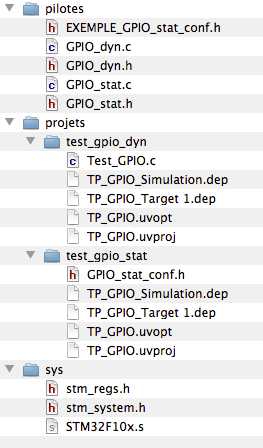
\includegraphics[width=0.35 \textwidth]{./figures/arborescence.png}
	\caption{Arborescence o� le r�pertoire \texttt{pilotes} est au m�me niveau que celui des projets. Plusieurs projets peuvent donc inclure le m�me pilote en donnant le chemin relatif vers le .h (\texttt{../../pilotes/GPIO\_stat.h}). Chaque applicatif de projet (\texttt{Test\_GPIO.c}) configure son pilote en passant les param�tres lors d el'appel de la fonction d'initialisation. Dans le cas de pilote statique, le fichier de configuration \texttt{GPIO\_stat\_conf.h} est plac� dans le projet car la configuration d�pend de l'application et ne peut �tre la m�me.}
	\label{fig:arbo}
 \end{SCfigure}

\subsection{Pilote statique}
Dans le cas statique, la configuration se fait directement dans un fichier de configuration, par exemple \texttt{./projet/exemple/GPIO\_stat\_conf.h}, appartenant au projet. Dans ce fichier de configuration, l'utilisateur va commenter ou d�commenter des directives \verb+#define ...+ :
  \begin{lstlisting}[float=htbp,frame=tb,caption = ./projet/exemple/GPIO\_stat\_conf.h : configuration via des directive de compilation]
//CONF : if you want to use GPIOA port then
// uncomment the following line
#define GPIOA_IS_USED

// CONF : by default all ports are inputs
// to set a port to output add lines in the format
// #undef P<port>_<pin>
// #define P<port>_<pin>  IS_OUTPUT
// Example : PB_3 fort pin number 3 of GPIOB
#undef PA_2
#define PA_2 IS_OUTPUT
\end{lstlisting}

Le fichier de configuration est inclus par le fichier source, par exemple \texttt{./pilotes/GPIO\_stat.c}, ce qui va influencer sa compilation et ainsi int�grer les configurations:
\begin{lstlisting}[float=htbp,frame=tb,caption = ./pilotes/GPIO\_stat.c : configur� via des directives de compilation]
#define IS_INPUT 0x0
#define IS_OUTPUT 0x3

#define PA_0 IS_INPUT
#define PA_1 IS_INPUT
#define PA_2 IS_INPUT
...

#include "GPIO_stat_conf.h"
// path to the conf file should be set in compiler options
// Now PA_x are configured by user

void GPIO_Init(void)
{
   #ifdef GPIOA_IS_USED
   // construct the init from the PA_x configured
   GPIOA->CRL = (PA_0<<0)|(PA_1<<4)|(PA_2<<8)|(PA_3<<12)|(PA_4<<16);
   #endif
}
\end{lstlisting}

L'application, quand � elle, ne fait qu'appeler une fonction d'initialisation sans param�tres :
\begin{lstlisting}[float=htbp,frame=tb,caption = ./projet/exemple/main\_stat.c : source applicative]
#include "../../../pilotes/GPIO_stat.h"
// ou #include "GPIO_stat.h" si le chemin est dans les options...
...
void main (void)
{
	Init_Clock();
	Init_GPIO();
}
\end{lstlisting}

Dans cet exemple la simplicit� n'est pas en faveur de la version statique, cependant le code produit statiquement est beaucoup moins co�teux en terme de m�moire, car il ne compilera les fonctions de configuration que si des ports sont utilis�s.

\section{Second exemple : configuration d'une interruption}

Les interruptions peuvent permettre d'ex�cuter une fonction li�e � l'application suite � un �v�nement mat�riel. Il y a donc d'un c�t� la fonction qui appartient � la couche applicative et de l'autre l'interruption � capturer au niveau de la couche pilotes. Lors de la configuration du syst�me il faut �tre capable de faire le lien entre ces deux �l�ments...
\subsection{Pilote dynamique}
Dans sa version dynamique, cela revient � prototyper une fonction dans le pilote du p�riph�rique qui permet de faire le lien entre la fonction et une interruption du p�riph�rique. Supposons que nous voulons ex�cuter la fonction \texttt{toto(void)} lors de l'interruption provoqu�e par le p�riph�rique \texttt{XXX}.

Le pilote de \texttt{XXX} comportera une fonction \texttt{Init\_IT\_XXX(void (* IT\_fonction) (void))} qui permettra de lier l'interruption de \texttt{XXX} � la fonction \texttt{IT\_fonction}.

\begin{lstlisting}[float=htbp,frame=tb,caption = ./pilotes/Pilote\_XXX.c : configuration d'une interruption]
void (*pt_IT_Hook) (void); // Pointeur de fonction pour l'IT

void Init_IT_XXX(void (* IT_fonction) (void))
{
	pt_IT_Hook = IT_fonction;
	... // Activer l'interruption
}
...
\end{lstlisting}

Le handler de l'interruption est alors d�fini dans la suite de mani�re g�n�rique par la code suivant :
\begin{lstlisting}[float=htbp,frame=tb,caption = ./pilotes/Pilote\_XXX.c : handler d'une interruption en dynamique]
...
void XXX_IRQHandler void // Handler de l'IT de XXX
{
 	if ((int) pt_IT_Hook != 0)
	{
		(*pt_IT_Hook)(); // Appel � la fonction
	}
}
\end{lstlisting}

Au niveau applicatif la configuration du p�riph�rique se fera gr�ce au code suivant :
\begin{lstlisting}[float=htbp,frame=tb,caption = ./projet/ex\_it/main.c : Exemple de configuration d'une interruption en dynamique]
#include "../../../pilotes/Pilotes_XXX.h"
...
void main (void) // Handler de l'IT de XXX
{
	Init_Clock();
	Init_GPIO();
 	Init_IT_XXX(&toto);
}

void toto(void)
{
	// Code � ex�cuter pendant l'interruption
}
...
\end{lstlisting}

Bien s�r la fonction de configuration de l'interruption pourrait �tre plus �volu�e, par exemple en fixant le niveau de l'interruption etc.

\subsection{Pilote statique}

Dans le cas d'un pilote statique la solution est plus simple � impl�menter. Il suffit de faire un fichier de configuration:
\begin{lstlisting}[float=htbp,frame=tb,caption = ./projet/exemple/Pilote\_XXX\_conf.h : configuration via des directive de compilation]
// CONFIGURATION PART
// please uncomment if you wich to launch a function on IT
// #define THERE_IS_A_HOOK_ON_IT
#ifdef THERE_IS_A_HOOK_ON_IT
	// CONFIGURE here the function prototype
	void toto (void);
	//CONFIGURE here the call to the hook function
	#define IT_HOOK_CALL  toto()
#endif
\end{lstlisting}

Le source du pilote utilise la directive \verb+#ifdef+ pour ins�rer ou non l'appel de la fonction lors de l'interruption
\begin{lstlisting}[float=htbp,frame=tb,caption = ./pilotes/Pilote\_XXX.c : handler d'IT utilisant les directives de compilation]
#include "Pilote_XXX_conf.h"
// path to the conf file should be set in compiler options

void XXX_IRQHandler void // Handler de l'IT de XXX
{
	#ifdef THERE_IS_A_HOOK_ON_IT
		IT_HOOK_CALL;
	#else
		...
	#end
	...
}
\end{lstlisting}

Remarquez que dans cet exemple, la version statique va g�n�rer uniquement un \emph{Handler} vide alors que la version dynamique g�n�re un \emph{Handler} avec 4 lignes de code, plus une fonction d'initialisation (1 ligne) et son appel du main (1 ligne). Vous comprenez maintenant la compacit� de la version statique mais malheureusement aussi sa complexit�...

\`A vous de choisir...


\chapter{Bah !  Les masques}
Pour programmer un p�riph�rique il est n�cessaire d'aller modifier un
ou plusieurs bits dans un registre sans modifier les autres. Par exemple le registre \verb+ADC_CR1+ sert � configurer le convertisseur analogique--num�rique \verb+ADC1+ :
\begin{figure}[htbp]
\begin{center}
\fbox{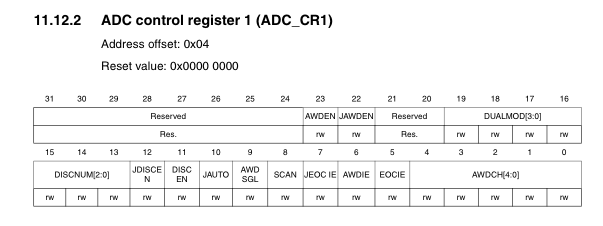
\includegraphics[width=\textwidth]{./figures/adc_cr1.png}}
\caption{Extrait du \emph{reference manual} du STM32 p. 236, la suite d�crit la fonction de chaque bit, comme \texttt{SCAN} et \texttt{AWDIE} et la signification des valeurs de chaque tranches de bit tels que \texttt{DISCNUM}}
\label{fig:adc_cr1}
\end{center}
\end{figure}


Pour cela on utilise les masques logiques et certaines astuces pour construire
un masque clairement sans risquer de se tromper. Dans l'exemple suivant le bit \texttt{SCAN} de \texttt{ADC\_CR1} est mis � 1 et le bit \texttt{EOCIE} est mis � 0 sans toucher aux autres bits.
Les registres \texttt{ADC1\_CR2}, \texttt{ADC1\_SQR1}, \texttt{ADC1\_SQR3} sont aussi manipul�s avec des masques~:

\begin{lstlisting}[frame=tb,caption = Extrait de la configuration de l'ADC de la baguette magique vue en assembleur]
ADC1->CR1  |= (ADC_SCAN);    // continuous scan of channels 1,14,15	

ADC1->CR1  &= ~(ADC_EOCIE);   // pas d'interruption de fin de conv.                                         

ADC1->CR2  |= (ADC_EXTSEL_ON_SWSTART | ADC_ CONT | ADC_DMA);  
    // EXTSEL = SWSTART 
    // use data align right,continuous conversion
    // send DMA request

// convert sequence is channel 1 then 14 then 15
ADC1->SQR3  |= (1 <<SQ1_SHIFT)  |  (14 <<SQ2_SHIFT) | (15 <<SQ3_SHIFT);                       
\end{lstlisting}


\begin{minipage}{0.5\linewidth}
	%\begin{figure}[htbp]
	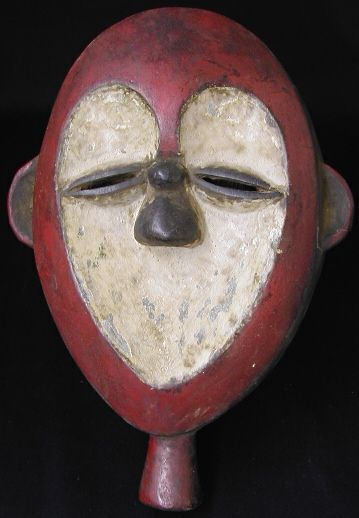
\includegraphics[width=0.6\textwidth]{./figures/masque_art_primitif.jpg}
	%\caption{}
	%\label{fig:art}
	%\end{figure}
\end{minipage}
\hfill
\begin{minipage}{0.5\linewidth}
Si vous avez aucune id�e de comment se code fonctionne c'est que vous ne maitrisez pas encore l'art primitif du masque~: lisez--donc la suite. 

\emph{Ci--contre, un masque primitif (on pr�f�re dire \emph{d'art premier}) d'origine Gabonaise.}
\end{minipage}

\section{Op�rateur logiques et bit � bit}
On utilise les op�rateurs  logiques ET, OU, XOR (OU exclusif) et NOT entre un registre et un masque pour manipuler les bits. Les op�rateurs logiques et leurs syntaxe en langage C sont r�sum�s dans le tableau suivant~:
\begin{center}
  \begin{tabular}{@{} c|c|c @{}}
    Fonction logique & Op�rateur logique & Op�rateur bit � bit \\ 
    \hline
    ET & \&\& & \& \\ 
    OU & || & | \\ 
    XOR & aucun & $\widehat{ }$ \\ 
    NON & ! & \ctilde \\ 
  
  \end{tabular}
\end{center}

L'op�rateur logique consid�re les op�randes (qu'elle soient 8/16/32 bit) comme une valeur bool�enne fausse si tous les bits sont nuls et vrai sinon. Elle fournit un r�sultat bool�en nul si c'est faux et diff�rent de z�ro (en g�n�ral la valeur 1) sinon. Ne confondez donc pas l'op�rateur logique avec l'op�rateur bit � bit qui effectue 8/16/32 op�rations logiques entre chaque bits respectifs des op�randes, par exemple :
\begin{lstlisting}[frame=tb]
a = 2; // soit b00000010 en binaire est vrai car diff�rent de 0
b = 1; // soit b00000001 en binaire est vrai aussi
y = a && b; // donne 1(vrai) car a ET b est vrai
z = a & b; // donne b00000000 car chaque ET des bits de a et b sont faux
\end{lstlisting}

\section{Mettre un bit � 1}

Pour cela on utilise l'op�rateur OU avec une valeur binaire, appel�e \emph{masque}, ayant des bits � 1 uniquement devant les bits que l'on veut initialiser~:
\begin{equation*}
\left.
\begin{array}{lcccccccc}
   & b_7 & b_6 & b_5 & b_4 & b_3 & b_2 & b_1 & b_0  \\
  OU\hspace{0.5cm} &0&0&0&1&0&0&1&1  \\
  \cline{2-9}
   = & b_7 & b_6 & b_5 &1& b_3 & b_2 &1&1  \\
\end{array}
\right.
\qquad \text{car } \quad x \,\, OU \,\, 1 = 1 \qquad \text{ et }\quad x \,\, OU \,\,0 = x
\end{equation*}

Ainsi les bits $b_4$, $b_1$ et $b_0$ sont pass�s � 1 sans modifier la valeur des autres bits.  

Pour effectuer cela en langage C on doit calculer la valeur du masque binaire : convertir  \texttt{b00010011} en hexad�cimal (\texttt{0x13}) ou en d�cimal (19) car le langage C n'admet pas de litt�raux en binaire.

\begin{lstlisting}[frame=tb]
char avoile;
...
//formulations �quivalentes
avoile = avoile |  0x13;   // op�rateur | inline
avoile |=  0x13;           // op�rateur | pr�fix� � =
avoile |=  19;             // valeur du masque en d�cimal
\end{lstlisting}

Il n'est pas tr�s �vident de comprendre que \texttt{0x13} ou \texttt{19} correspond � un masque visant les bits de rang $0$,$1$ et $4$, de plus il est tr�s facile de se tromper lorsque l'on fait la conversion soi--m�me. Un \emph{geek} utilisera l'op�rateur de d�calage � gauche \verb+<<x+ pour positionner un 1 devant  le bit de rang $x$ pour construire sont masque ainsi~:
\begin{equation*}
\left.
\begin{array}{lrccccccccc}
&                &                      & b_7 & b_6 & b_5 & b_4 & b_3 & b_2 & b_1 & b_0  \\
& (1<<0)   & \rightarrow &  0&0&0&0&0&0&0&1  \\
OU & (1<<1)   & \rightarrow &  0&0&0&0&0&0&1&0  \\	 
OU &  (1<<4)   &  \rightarrow &  0&0&0&1&0&0&0&0  \\	
 \cline{4-11} 
 = & (1<<0)|(1<<1)|(1<<4)   &  \rightarrow &  0&0&0&1&0&0&1&1  \\	
\end{array}
\right.
\end{equation*}
 
Ainsi le code suivant est plus lisible et ne risque pas de comporter d'erreur de conversion~:
\begin{lstlisting}[frame=tb]
//formulations �quivalentes
avoile = avoile |  0x13;   // op�rateur | inline
avoile = avoile | (1<<0)|(1<<1)|(1<<4);
avoile |= (1<<0)|(1<<1)|(1<<4);
\end{lstlisting}

\section{Mettre un bit � 0}

Pour cela on utilise l'op�rateur ET avec une masque ayant des bits � 0 uniquement devant les bits que l'on veut initialiser~:
\begin{equation*}
\left.
\begin{array}{lcccccccc}
   &b_7& b_6 & b_5 & b_4 & b_3 & b_2 & b_1 & b_0  \\
  ET\hspace{0.5cm} &1&1&1&0&1&1&0&0  \\
    \cline{2-9}
   = & b_7 & b_6 & b_5 &0& b_3 & b_2 &0&0  \\
\end{array}
\right.
\qquad \text{car } \quad x \,\, ET \,\, 1 = x \qquad \text{ et }\quad x \,\, ET \,\,0 = 0
\end{equation*}

Ainsi les bits $b_4$, $b_1$ et $b_0$ sont pass�s � 0 sans modifier la valeur des autres bits.  


Pour construire le masque, on peut toujours effectuer la conversion soit-m�me avec un risque d'erreur~: $b11101100 = 0xEC = 236$. On peut aussi construire le masque avec des 1 devant les bits � annuler et ensuite inverser chaque bit avec l'op�rateur \ctilde.
\begin{equation*}
\left.
\begin{array}{lrccccccccc}
  & (1<<0)|(1<<1)|(1<<4)   &  \rightarrow &  0&0&0&1&0&0&1&1  \\	
  & \ctilde(1<<0)|(1<<1)|(1<<4)   &  \rightarrow &  1&1&1&0&1&1&0&0  \\	
ET &   \mbox{avoile}            &   \rightarrow  & b_7 & b_6 & b_5 & b_4 & b_3 & b_2 & b_1 & b_0  \\
\cline{4-11}
 = &  \mbox{avoile }  \, \& \ctilde\!\!\!\!( (1<<0)|(1<<1)|(1<<4) )  &  \rightarrow & b_7 & b_6 & b_5 &0& b_3 & b_2 &0&0  \\
\end{array}
\right.
\end{equation*}

Ce qui donne en langage C :
\begin{lstlisting}[frame=tb]
//formulations �quivalentes
avoile = avoile &  0xEB;   
avoile = avoile & ~((1<<0)|(1<<1)|(1<<4));
avoile &= ~((1<<0)|(1<<1)|(1<<4));
\end{lstlisting}

\section{Inverser un bit}

Pour cela on utilise l'op�rateur XOR avec une masque ayant des bits � 1 uniquement devant les bits � inverser~:
\begin{equation*}
\left.
\begin{array}{lcccccccc}
   &b_7& b_6 & b_5 & b_4 & b_3 & b_2 & b_1 & b_0  \\
  XOR \hspace{0.5cm}  &0&0&0&1&0&0&1&1  \\
   \cline{2-9}
   =&b_7& b_6 & b_5 &\overline{b_4}& b_3 & b_2 &\overline{b_1}&\overline{b_0}  \\
\end{array}
\right.
\qquad \text{car } \quad x \,\, XOR \,\, 1 = \overline{x} \qquad \text{ et }\quad x \,\, XOR \,\,0 = x
\end{equation*}

Ainsi seuls les bits $b_4$,$b_1$ et $b_0$ ont �t� invers�s.

On construit les masques comme les masque OU de mise � 1.

\section{Initialiser une tranche de bits}
Une tranche de bit est un ensemble de quelques bits contigus dont la valeur a une signification particuli�re. Par exemple \texttt{DISCNUM} est une tranche de 3 bits du registre \texttt{ADC\_CR1} qui indique le nombre de canaux � convertir.

Un programmeur avertis peut d�sirer initialiser une tranche de \texttt{avoile} � la valeur contenue dans \texttt{numero}. Pour cela il faut proc�der en trois �tapes~: limiter la valeur de \texttt{numero} pour ne pas d�passer la tranche de 3 bits et la caler au bon endroit ; annuler la tranche de trois bits de \texttt{avoile} ; puis recopier les 1 du premier masque dans \texttt{avoile} avec un OU~:
\begin{equation*}
\left.
\begin{array}{lrccccccccc}
  & \mbox{num}   &  \rightarrow &   n_7 & n_6 & n_5 & n_4 & n_3 & n_2 & n_1 & n_0  \\ 
  &  0x7   &  \rightarrow &   0&0&0&0&0 &1&1&1 \\ 
  & (\mbox{num} \, \& \, 0x7)   &  \rightarrow &  0&0&0&0&0 & n_2 & n_1 & n_0  \\ 
  & (\mbox{num} \, \& \, 0x7)<<4   &  \rightarrow &  0 & n_2 & n_1 & n_0 & 0 & 0 & 0 & 0  \\ 
OU &   \mbox{avoile}  \, \& \ctilde\!\!\!\!(0x7 << 4)           &   \rightarrow  & b_7 & 0 & 0 & 0 & b_3 & b_2 & b_1 & b_0  \\
\cline{4-11}
 = &  (\mbox{avoile} \, \, \& \ctilde\!\!\!\!(0x7 << 4) )  \, | \,(\mbox{num}\, \&\, 0x7)<<4)  &  \rightarrow & b_7 & n_2 & n_1 &n_0& b_3 & b_2 &b_1&b_0  \\
\end{array}
\right.
\end{equation*}


Le programme suivant permet d'affecter la tranche \texttt{DISCNUM} avec la valeur contenue dans la variable \texttt{numero}~:
\begin{lstlisting}[frame=tb]
void set_discnum ( char numero)
{
   // raz de la tranche DISCNUM : 3 bits de rang 13-15 de ADC_CR1
   ADC->CR1 &= ~(0x7<<13); // seuls les bits 13-15 du masque valent 0
   
   // init de la tranche avec numero
   ADC->CR1 |= numero<<13 // recopie les 1 de numero d�cal� au rang 13
   
   //Attention si numero >7 �a d�borde sur les bits 16 � 31
   //Un masque doit limiter numero de 0 � 7 : pas plus de trois bits � 1
   // On pr�f�re donc cette ligne
   ADC->CR1 |= (numero & 0x7) <<13 // numero est limit�
 }
\end{lstlisting}



%\chapter{Etape 1 : GPIO}

\begin{minipage}{0.2\linewidth}
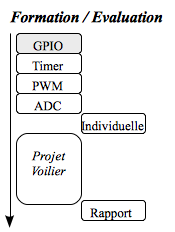
\includegraphics[width=\textwidth]{./figures/etape_gpio.png}
\end{minipage}
\hfill
\begin{minipage}{0.7\linewidth}
Les \emph{General Purpose Input Output (GPIO) ports} sont les p�riph�riques les plus simples � comprendre.
Les comp�tences vis�es sont~:
\begin{itemize}
\item savoir trouver une information dans la bonne doc
\item comprendre l'�tape de configuration d'un p�riph�rique
\item programmer un port d'E/S
\item concevoir un pilote �l�mentaire un peu g�n�rique
\end{itemize}
\end{minipage}

%____________________________________________________________
\section{Le GPIO dans le syst�me~: Bordage de voile automatique d'un voilier}

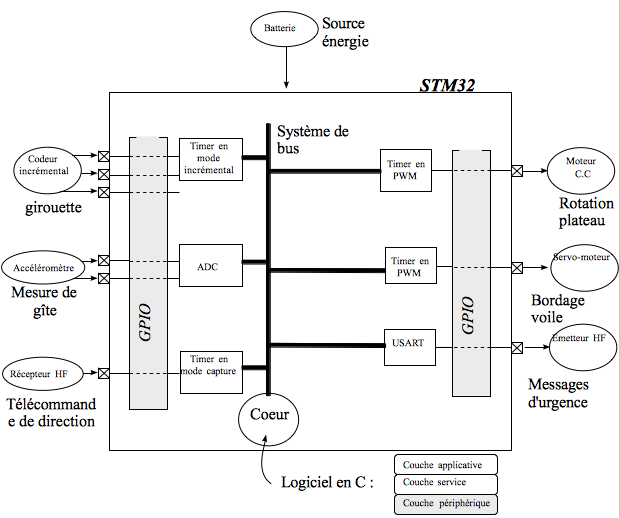
\includegraphics[width=0.8\textwidth]{./figures/system_gpio.png}

%____________________________________________________________
\section{Les ports d'E/S en g�n�ral}

Un port d'entr�e/sortie communique avec l'ext�rieur du micro-contr�leur par le biais de plusieurs fils (broches), en g�n�ral regroup� par paquet de 8 ou 16. Il communique avec le processeur par sa seule et unique possibilit� : les bus d'adresses et de donn�es. Ceci est commun � TOUS les p�riph�riques du micro--contr�leur. 
Par voie de cons�quence, tout p�riph�rique poss�de en son sein un certain nombre de registres accessibles en lecture ou �criture par le coeur. Ceux-ci on pour r�le de configurer et d'utiliser le p�riph�rique.


Un port d'E/S a donc pour r�le d'imposer (Output) ou de lire (Input) un niveau de tension  (associ� aux niveaux logique $0$ ou $1$ )  sur l'ensemble de ses broches. Selon le micro--contr�leur, le niveau logique $1$ peut �tre $5V$, $3V3$ ou encore $1V8$.


Le port d'E/S poss�de donc au minimum deux registres de configuration (l'un qui sp�cifie pour chaque broche sa direction, l'autre sp�cifiant la technologie utilis�e) et un registre d'utilisation qui est � l'image logique des broches.

\subsubsection{Technologie de sortie}
\begin{figure}[h!]
\begin{minipage}{0.48\linewidth}
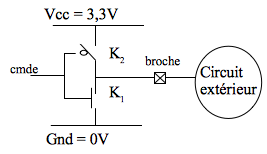
\includegraphics[width=0.9\textwidth]{./figures/gpio_push_pull.png}
%\caption

{\emph{Push--Pull}\footnote{Pousse--tire}-- La structure (technologie) poss�de deux interrupteurs (K1, K2, des transistors MOS compl�mentaires). K1 et K2 sont syst�matiquement invers�s : La broche peut donc �tre port�e au potentiel 0V ou 3,3V.
En mode \emph{Push--Pull}, c'est le port d'E/S qui impose le niveau logique d'une broche, que ce soit un niveau $1$ ou $0$. Il est le ma�tre, le circuit ext�rieur est l'esclave, r�cepteur.}
\end{minipage}
\hfill
\begin{minipage}{0.48\linewidth}
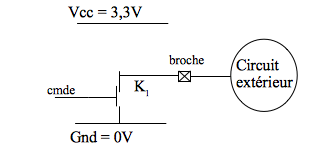
\includegraphics[width=\textwidth]{./figures/gpio_open_drain.png}
%\caption[]

{\emph{Open Drain}\footnote{Drain ouvert~: drain est le nom de la broche du transistor MOS reli�e � la broche : \og Drain laiss� ouvert\fg{}}-- Ici, un seul int�rrupteur est command�, l'autre est maintenu bloqu� (on ne le fait pas appara�tre): la broche ne peut �tre port�e par le port qu'� une tension de 0V.
Remarquons que si K1 est ouvert, la broche est \og en l'air \fg{}. Ce sera donc au circuit ext�rieur de fixer le potentiel de la broche dans cet �tat pr�cis. En mode \emph{Open Drain}, le port d'E/S ne peut imposer que le niveau logique $0$. Le niveau $1$ est fix� par le circuit ext�rieur. Le port d'E/S n'est donc pas le seul ma�tre du potentiel sur la broche. Le circuit ext�rieur l'est aussi.}
\end{minipage}
\end{figure}



\subsubsection{Technologie d'entr�e}
%\begin{figure}[h!]
\begin{minipage}{0.45\linewidth}
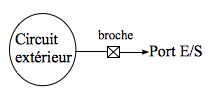
\includegraphics[width=0.8\textwidth]{./figures/gpio_floatting.png}
%\caption

{\emph{floating input}\protect\footnote{entr�e flottante} --
La broche, c�t� du port E/S, est laiss�e libre, flottante. Ainsi, c'est le circuit ext�rieur qui est totalement ma�tre du potentiel de la broche. Cela veut aussi dire, que si le circuit ext�rieur est d�connect�, le broche poss�de un potentiel inconnu (� proscrire car favorise le captage de parasites).}
\end{minipage}
\hfill
\begin{minipage}{0.45\linewidth}
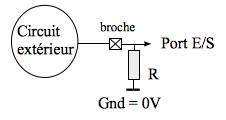
\includegraphics[width=0.8\textwidth]{./figures/gpio_pull_down.png}
%\caption

{\emph{Pull Down/Up}\protect\footnote{entr�e tir�e au niveau bas/haut} --
Dans le \emph{pull down}, une r�sistance (dite de rappel) relie la broche au 0V. Le potentiel de la broche se retrouve ainsi � 0V lorsque le circuit ext�rieur est d�connect�. Le circuit ext�rieur peut imposer un potentiel � condition d'avoir une r�sistance de sortie faible devant R. M�me principe pour le \emph{pull up}, mais la r�sistance est reli�e au Vcc ($5V$, $3V3$, ou $1V8$)
}
\end{minipage}
%\end{figure}


\section{� faire}

Afin de r�aliser les programmes logiciel de couche basse (p�riph�rique), le programmeur doit avoir une connaissance solide du micro--contr�leur cible. Ainsi, la premi�re t�che est de chercher les informations n�cessaires dans une documentation constructeur. Cette �tape, longue, sera tout de m�me facilit�e par les connaissances apport�es au chapitre pr�c�dant.

La documentation � disposition :
\begin{description}
\item[PM0056 Programming manual :]  document ST qui d�crit le coeur Cortex M3, et en particulier les instruction assembleur mais aussi les p�riph�riques natifs du coeur que sont le gestionnaire d'interruption, NVIC, et le timer syst�me, SYSTICK. (STM32\_PM0056.pdf)
\item[RM0008 Reference manual] document ST qui d�crit les p�riph�riques de la famille des STM32F103xx, qui donne toutes les informations utiles au sujet des p�riph�riques de la puce.
\item[STM32F103x6, STM32F103x8, STM32F103xB] \emph{datasheet} du micro--contr�leur qui traite de tout ce qui est limitation de vitesse, contraintes �lectrique, bo�tier...
\end{description}


M�thodologie g�n�rale de lecture du \emph{reference manual} :
\begin{enumerate}
\item S'approprier le p�riph�rique : Il faut identifier, dans le chapitre qui traite du p�riph�rique �tudi�, sa structure, son fonctionnement, en s'appuyant sur que l'on sait d�j� de ce type de circuit. Pour cela, tr�s souvent on trouve un sch�ma fonctionnel qui aide beaucoup. 
\item Identifier les registres qui sont n�cessaires au fonctionnement du p�rph�rique, identifier les champs de bit dans chacun des registres qui ont une fonction de configuration int�ressante pour l'application donn�e.
\item Noter en commentaire dans les fichiers .c ces informations avant m�me de commencer � �crire le module de la couche driver.
\end{enumerate}

 
\subsection{Questionnaire guide}

Nous allons travailler sur le micro--contr�leur dont la r�f�rence est STM32F103RB, en bo�tier LQFP64.

\paragraph{Q1~:} Donner le nombre de port GPIO de la puce, et pour chacun d'entre eux donner le nombre de broches associ�es

\paragraph{Q2~:} Trouver le nom des registres associ�s aux fonctions suivante et indiquez, pour chacun, s'il sert � configurer le port ou � communiquer :

\begin{tabular}{|c|c|c|}
\hline
Fonction du registre & Nom du registre & Config. ou comm. \\ \hline
Permet de fixer la direction des broches du port & & \\ \hline
Permet du fixer la technologie de chaque broche& & \\ \hline
Contient l'image du port en lecture& & \\ \hline
Contient l'image du port en �criture& & \\ \hline
\end{tabular}

\paragraph{Q3~:} Expliquer � quoi sert le registre GPIOx.BSRR

\paragraph{Q4~:} D�cliner toutes les possibilit�s technologiques des broches du GPIO. Sur quel champ de registre doit-on agir pour faire le choix ?

\paragraph{Q5~:} Qu'appelle t-on Alternate function ?


\subsection{Projets Keils � r�aliser}
\subsubsection{Premiers pas}
En premi�re �tape, vous allez concevoir l'�quivalent du \og hello world\fg{} pour les p�riph�riques : le \emph{blinky}. 
Pour cela r�cup�rez les fichier \texttt{src\_etudiants.zip} sur le wiki et d�compressez-le dans votre r�pertoire favori.

Les r�pertoires~:
\begin{description}
\item[sys] contient les fichiers .h n�cessaires � la d�finition des registres (\texttt{stm\_regs.h}), ainsi que le fichier de d�marrage �crit en assembleur.
\item[pilotes] contiendra bien s�r les pilotes tels que le module \texttt{GPIO.c} et son ent�te \texttt{GPIO.h}.
\item[projet] contient des r�pertoire de projets applicatifs comme \texttt{premiers\_pas}. Chaque r�pertoire projet contiens au moins un fichier \texttt{.uvproj} et les sources applicatives comme \texttt{main.c} 
\end{description}

Ouvrez le projet contenu dans  \texttt{./projets/premiers\_pas} et compl�tez le \texttt{main.c} afin de faire clignoter (aussi vite que vous voudrez) la diode branch�e sur le port GPIOB broche 9. Vous utiliserez pour cela les masques binaires et la d�finition des registres de \texttt{./sys/stm\_regs.h}. Mesurez la p�riode d'oscillation � l'oscilloscope et tentez d'identifier le nombre de cycles machines utilis�s. 

Le \texttt{main.c} que vous avez r�alis� est typiquement un exemple de fichier m�langeant les couches pilotes et application. On vous demande dans la suite d'�crire un pilote des ports GPIO g�n�rique et de l'utiliser dans cette application. 

\subsubsection{Premier pilote}
Cr�ez un nouveau projet dans \texttt{./projets/test\_GPIO/} � partir de z�ro. Vous r�digez le module \texttt{./pilotes/GPIO.c}  correspondant � son API, \verb+GPIO.h+ (qui vous est donn�e en guise de sp�cification). L'applicatif de test, par exemple \texttt{./projets/test\_gpio/main\_blinky.c}, doit permettre de d�boguer le module, et d'y op�rer des tests le plus complets possibles en d�marrant par le simple ��blinky��.

Le travail qui vous est demand� (tout comme ceux des futurs TP) est ainsi directement r�utilisable pour le projet voilier.









\end{document}

